\clearpage

\section{Balanced Photodetector}

\begin{tcolorbox}	
	\begin{tabular}{p{2.75cm} p{0.2cm} p{10.5cm}} 	
		\textbf{Header File}   &:& photodiode\_old.h \\
		\textbf{Source File}   &:& photodiode\_old.cpp \\
        \textbf{Version}       &:& 20190403 (\emph{Jorge Ribeiro})\\
	\end{tabular}
\end{tcolorbox}


The Balanced Photodetector (BPD) measures the broadband difference signal of two photodiodes. It can be used as a low noise receiver in optical experiments.

It works a photodiode pair, two photodiodes assembled. It accepts two optical signals and the output is one electrical signal.


\begin{figure}[h]
	\centering\includegraphics[width=0.5\textwidth]{./lib/photodiode/figures/photodiode.png}
	\caption{Schematic representation of the physical equivalent of the photodiode code block.}\label{photodiode}
\end{figure}

In the simplified schematic representation of the Homodyne Receiver block, the balanced photodetector or photodiode pair can be found between the optical hybrid and the TI Amplifier.

\subsection*{Input Parameters}

\begin{itemize}
	\item responsivity\{1\}
	\item thermal Noise Amplitude\
\end{itemize}

\subsection*{Methods}

BalancedPhotodetector () {}
\bigbreak
BalancedPhotodetector($initializer_list$$<$Signal *$>$ InputSig, $initializer_list$$<$Signal *$>$ OutputSig) :Block(InputSig, OutputSig) {}
\bigbreak
void initialize(void)
\bigbreak
bool runBlock(void)
\bigbreak
void setResponsivity(\texttt{$t\_real$} Responsivity)
\bigbreak
void setThermalNoiseAmplitude($t_real double amplitude$)

\subsection*{Functional description}

This block accepts two input optical signals. It computes the optical power of the signal (given by the absolute value squared of the input signal) and multiplies it by the responsivity of the photodiode. This product corresponds to the current generated by the photodiode. This is done for each of the input signals. The two currents are then subtracted producing a single output current, that originates the output electrical signal of the block.

\subsection*{Input Signals}

\subparagraph*{Number:} 2

\subparagraph*{Type:} Optical (OpticalSignal)

\subsection*{Output Signals}

\subparagraph*{Number:} 1

\subparagraph*{Type:} Electrical (TimeContinuousAmplitudeContinuousReal)


\subsection*{Examples}

According to the simplified schematic representation of the Homodyne Receiver block the two originals signals S6 and S7 enter the Optical Hybrid, transform into 4 optical signals that enter the two photodetectors and correspond to two electrical signals shown below.

\begin{figure}[h]
	\centering
	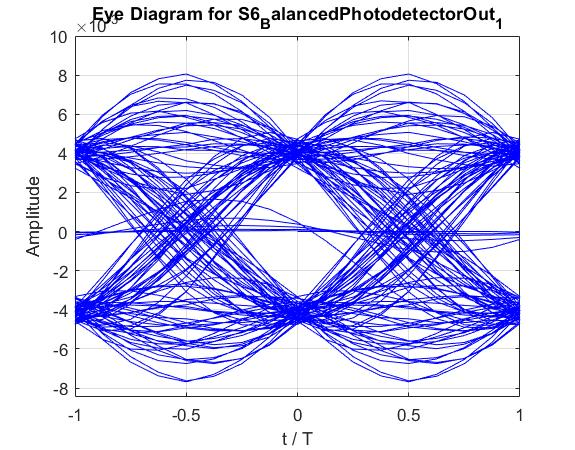
\includegraphics[width=\textwidth]{./lib/photodiode/figures/S6_BalancedPhotodetectorOut_1_EyeDiagram}
	\caption{Eye diagram for the S6 output of the Photodetector.}
\end{figure}

\begin{figure}[h]
	\centering
	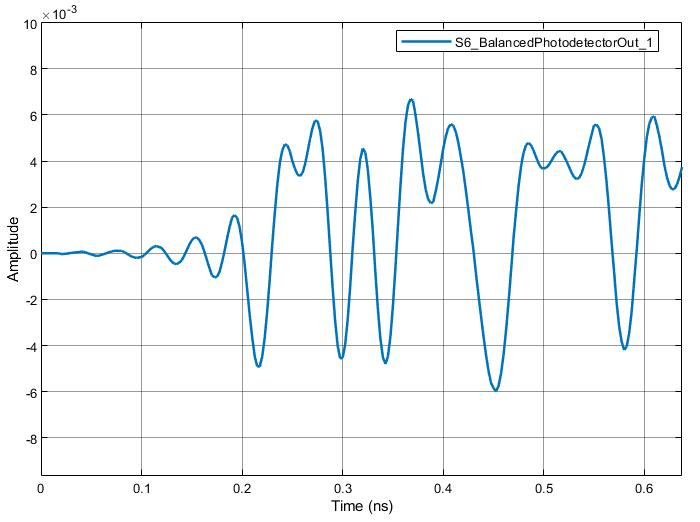
\includegraphics[width=\textwidth]{./lib/photodiode/figures/S6_BalancedPhotodetectorOut_1_time}
	\caption{Amplitude vs Time for the S6 output of the Photodetector.}
\end{figure}

\begin{figure}[h]
	\centering
	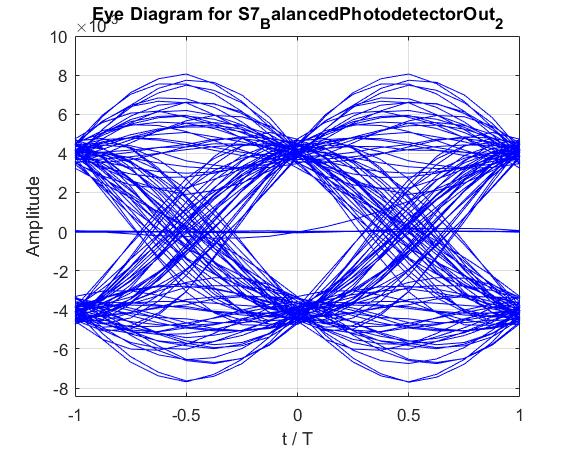
\includegraphics[width=\textwidth]{./lib/photodiode/figures/S7_BalancedPhotodetectorOut_2_EyeDiagram}
	\caption{Eye diagram for the S7 output of the Photodetector.}
\end{figure}

\begin{figure}[h]
	\centering
	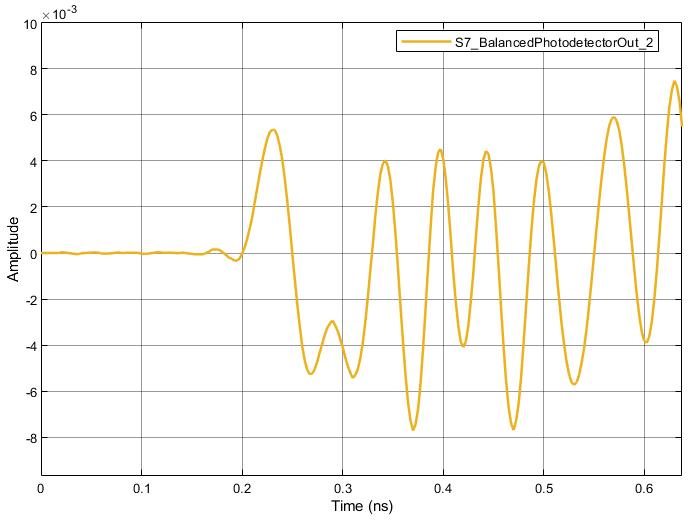
\includegraphics[width=\textwidth]{./lib/photodiode/figures/S7_BalancedPhotodetectorOut_2_time}
	\caption{Amplitude vs Time for the S7 output of the Photodetector.}
\end{figure}


\subsection*{Sugestions for future improvement}

